
\section*{1. Uso cotidiano de la PC}
La PC se utiliza principalmente para el desarrollo de software y la ejecución de simulaciones. Los programas y entornos utilizados incluyen:
\begin{itemize}
    \item \textbf{Desarrollo de software:} Visual Studio Code, PyCharm, Eclipse.
    \item \textbf{Simulaciones:} MATLAB, Simulink, ANSYS.
    \item \textbf{Otros:} Navegación web con múltiples pestañas, edición de documentos en \LaTeX.
\end{itemize}

\section*{2. Tareas y benchmarks representativos}

A continuación, se presenta una tabla con algunas tareas frecuentes relacionadas con simulaciones y desarrollo de código, junto con el benchmark que mejor representa cada una.

\begin{center}
\begin{tabular}{|p{7cm}|p{7cm}|}
\hline
\textbf{Tarea} & \textbf{Benchmark representativo} \\
\hline
Compilar proyectos grandes en C/C++ & Geekbench o Cinebench (CPU multi-core) \\
\hline
Ejecución de simulaciones en MATLAB/Simulink & SPEC CPU2017 \\
\hline
Desarrollo de software en entornos pesados (e.g., PyCharm, Eclipse) & PassMark CPU \\
\hline
Análisis de datos y cálculos intensivos en Python & Geekbench (CPU single-core) \\
\hline
\end{tabular}
\end{center}

Ahora veremos algunos resultados, comenzando por el de Geekbench, que hace una revisión general de varios aspectos de mi PC.

Siendo estas las características de mi computadora:

\begin{figure}[H]
    \centering
    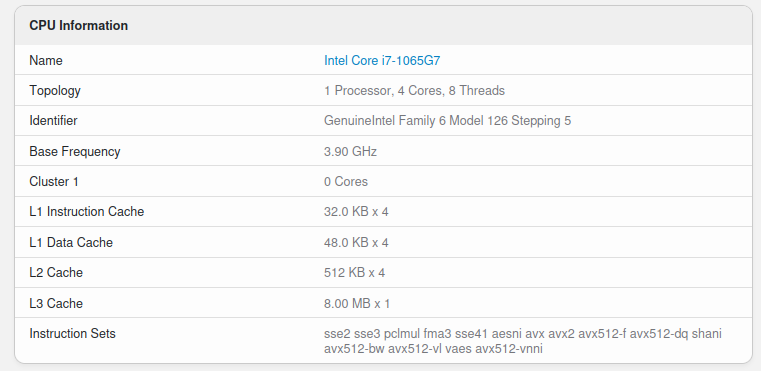
\includegraphics[width=0.7\linewidth]{img/sistema.png}
    \caption{Prestaciones}
    \label{fig:enter-label}
    
\end{figure}
dio como resultado general lo siguiente
\begin{figure}[H]
    \centering
    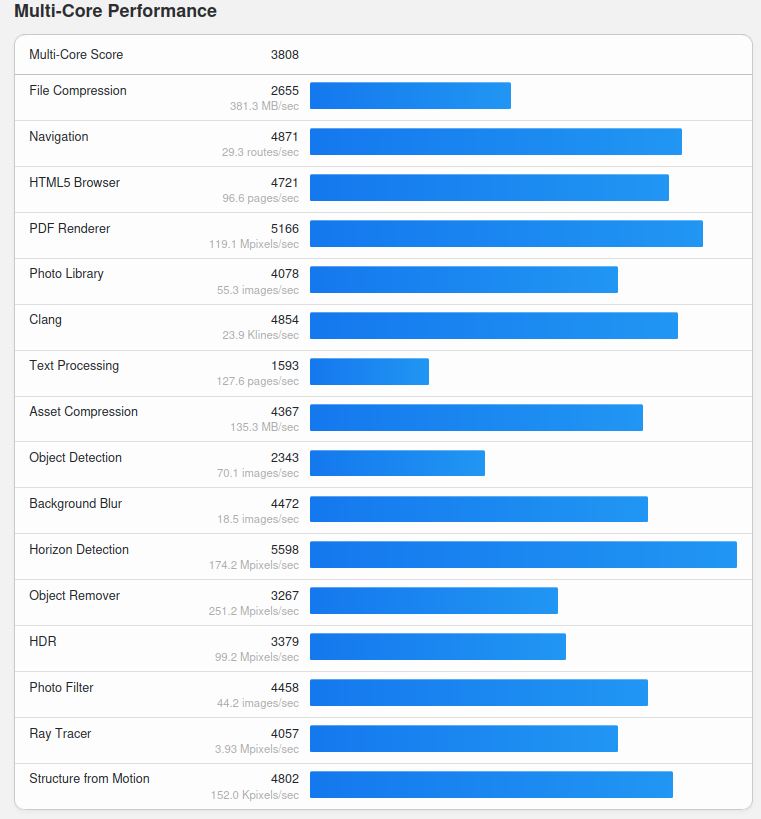
\includegraphics[width=0.7\linewidth]{img/rendimientoGeek.png}
    \caption{Resultado}
    
\end{figure}

\begin{figure}[H]
    \centering
    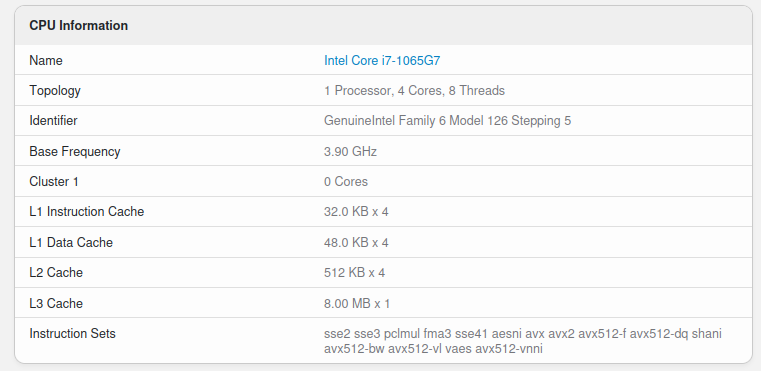
\includegraphics[width=0.7\linewidth]{img/sistema.png}
    \caption{Prestaciones}
    \label{fig:enter-label}
\end{figure}
dio como resultado general lo siguiente:
\begin{figure}[H]
    \centering
    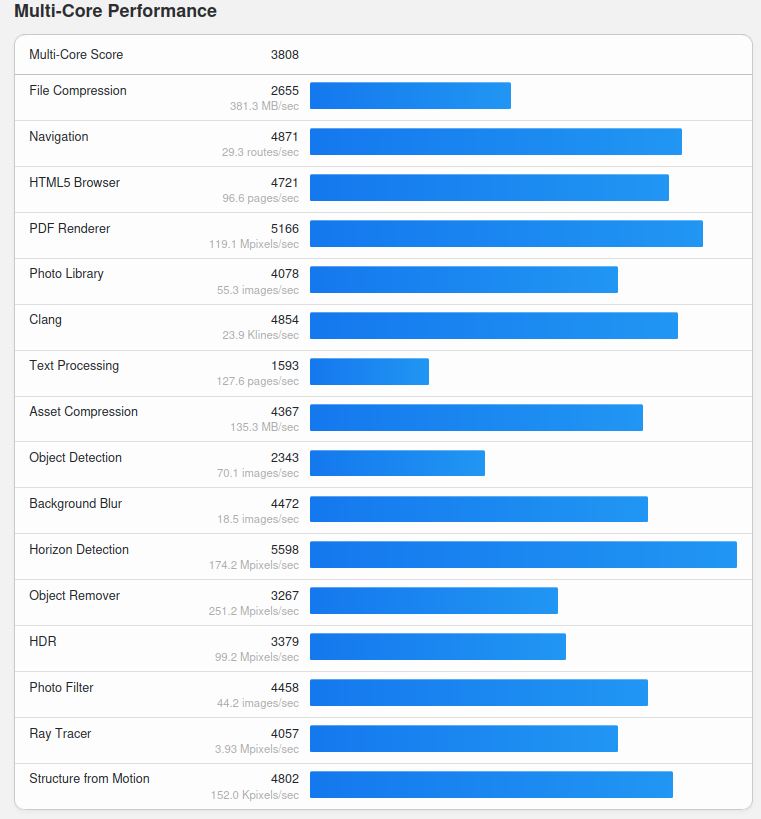
\includegraphics[width=0.7\linewidth]{img/rendimientoGeek.png}
    \caption{Resultado}
\end{figure}

Como se puede ver, tengo buenos rendimientos en detección horizontal y muy buenas respuestas en navegación y manejo de PDF e imágenes. Estos resultados podrían verse afectados debido a que, mientras realizaba este benchmark, también realizaba la instalación de un programa en mi computadora.

Luego tuvimos problemas a la hora de correr otros benchmarks, debido a que la mayoría son pagos (SPEC CPU2017) o no corren en la versión actual de Ubuntu (PassMark CPU), por lo que dejaremos este análisis hasta aquí.

\section*{3. Reflexión final}
En términos generales, la PC cumple con los requerimientos diarios para el desarrollo de software y la ejecución de simulaciones. Sin embargo, se ha identificado que el rendimiento de la CPU puede convertirse en un cuello de botella durante la ejecución de simulaciones complejas y la compilación de proyectos grandes.
